% ===================================
% CODICE LaTeX PER GRAFICI E TABELLE
% Tesi GDO - Capitoli 1 e 2
% ===================================
% filepath: c:\Users\saint\tesi\nuovi grafi 1 e 2.tex
\documentclass[border=10pt]{standalone}
% Pacchetti necessari
\usepackage[utf8]{inputenc}
\usepackage[T1]{fontenc}
\usepackage{amsmath}
\usepackage{amssymb}    
\usepackage{graphicx}
\usepackage{caption}
\usepackage{subcaption} % Per sottotitoli nelle figure
% Preambolo necessario:
\usepackage{tikz}
\usepackage{pgfplots}
\usepackage{booktabs}
\usepackage{multirow}
\pgfplotsset{compat=1.17}
\usetikzlibrary{pgfplots.polar}

% ===================================
% CAPITOLO 1
% ===================================
\begin{document}
% FIGURA 2.5: Framework Integrato di Sicurezza GDO

\centering
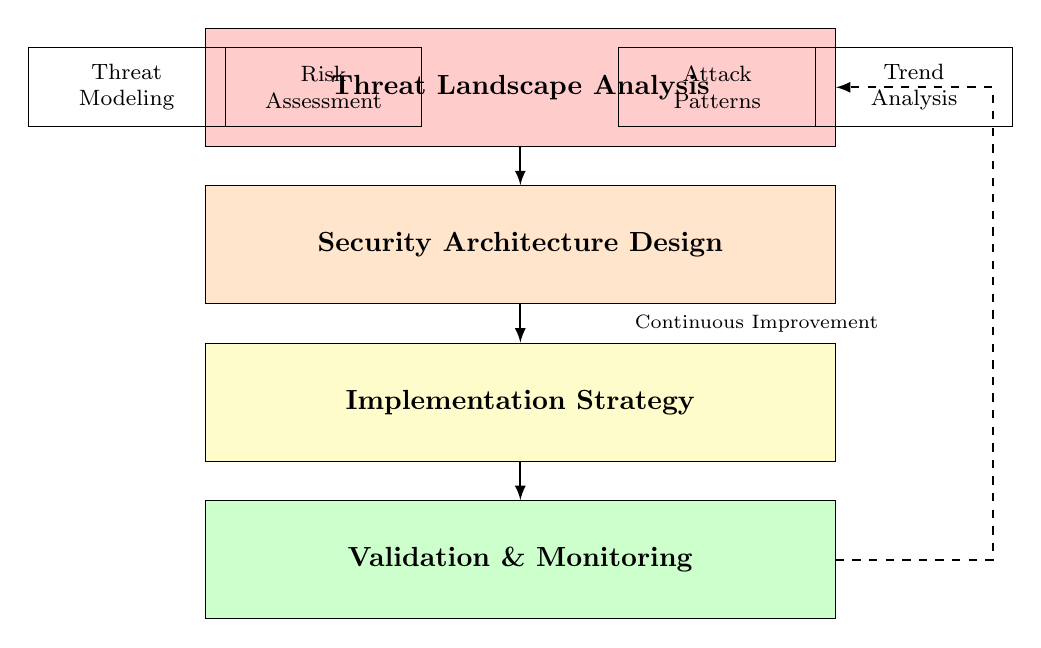
\begin{tikzpicture}[
    level/.style={rectangle, draw, text centered, minimum width=8cm, minimum height=1.5cm},
    component/.style={rectangle, draw, text centered, minimum width=2.5cm, minimum height=1cm, font=\footnotesize},
    arrow/.style={->, thick, >=latex}
]

% Livelli principali
\node[level, fill=red!20] (threat) at (0,0) {\textbf{Threat Landscape Analysis}};
\node[level, fill=orange!20] (arch) at (0,-2) {\textbf{Security Architecture Design}};
\node[level, fill=yellow!20] (impl) at (0,-4) {\textbf{Implementation Strategy}};
\node[level, fill=green!20] (valid) at (0,-6) {\textbf{Validation \& Monitoring}};

% Componenti
\node[component, align=center] (t1) at (-5,0) {Threat\\Modeling};

\node[component, align=center] (t2) at (-2.5,0) {Risk\\Assessment};
\node[component, align=center] (t3) at (2.5,0) {Attack\\Patterns};
\node[component, align=center] (t4) at (5,0) {Trend\\Analysis};

% Frecce di flusso
\draw[arrow] (threat) -- (arch);
\draw[arrow] (arch) -- (impl);
\draw[arrow] (impl) -- (valid);

% Feedback loop
\draw[arrow, dashed] (valid.east) -- ++(2,0) -- ++(0,6) -- (threat.east);
\node[font=\scriptsize] at (3,-3) {Continuous Improvement};

\end{tikzpicture}


\end{document}
% --- IGNORE ---